\bookchapter{Collections: Lists, Dictionaries and Sets}\label{ch:py4}

\section*{Explanation}
A robot has $23$ joints, a camera delivers thousands of pixels, a log has thousands of lines. You cannot give every value its own variable. A \textbf{collection} holds many values under one name. Python has four main ones, and choosing the right one is half of a good program:
\begin{center}
\renewcommand{\arraystretch}{1.25}
\begin{tabular}{p{2.2cm}p{3.2cm}p{7.6cm}}
\textbf{Type} & \textbf{Example} & \textbf{Properties}\\ \hline
\texttt{list} & \texttt{[3, 1, 4]} & ordered, changeable, duplicates allowed\\
\texttt{tuple} & \texttt{(1.5, 2.0)} & ordered, \emph{not} changeable; for small fixed groups such as a point\\
\texttt{dict} & \texttt{\{"hip": 0.1\}} & maps \textbf{keys} to values; fast lookup by key\\
\texttt{set} & \texttt{\{1, 2, 3\}} & no duplicates, no order; fast ``is it in there?''\\
\end{tabular}
\end{center}

\section*{Lists}
\begin{center}
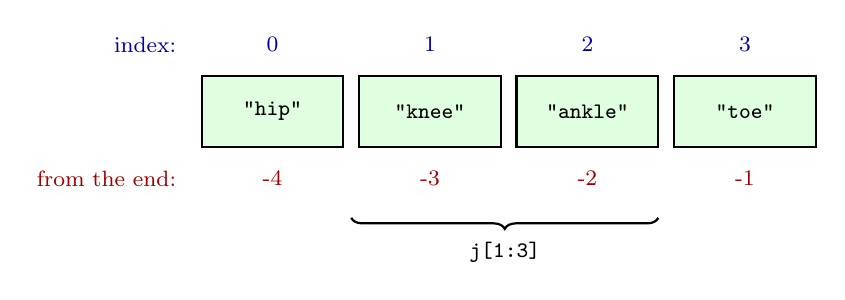
\begin{tikzpicture}
  \foreach \i/\t in {0/hip,1/knee,2/ankle,3/toe}{
    \node[draw,thick,minimum width=1.8cm,minimum height=0.9cm,fill=green!12,font=\footnotesize\ttfamily] at (2*\i,0) {"\t"};
    \node[font=\footnotesize,blue!60!black] at (2*\i,0.85) {\i};
  }
  \foreach \i/\n in {0/-4,1/-3,2/-2,3/-1}{
    \node[font=\footnotesize,red!60!black] at (2*\i,-0.85) {\n};
  }
  \node[font=\footnotesize,blue!60!black,anchor=east] at (-1.1,0.85) {index:};
  \node[font=\footnotesize,red!60!black,anchor=east] at (-1.1,-0.85) {from the end:};
  \draw[decorate,decoration={brace,amplitude=4pt,mirror},thick] (1.0,-1.35)--(4.9,-1.35) node[midway,below=5pt,font=\footnotesize\ttfamily]{j[1:3]};
\end{tikzpicture}
\captionof{figure}{A list of four elements. Indices count from $0$, negative indices from the end. The slice \texttt{j[1:3]} contains the elements $1$ and $2$ (the end is excluded).}\label{fig:py4_list}
\end{center}
\begin{verbatim}
>>> j = ["hip", "knee", "ankle", "toe"]
>>> j[0], j[-1], j[1:3], j[::2], len(j)
('hip', 'toe', ['knee', 'ankle'], ['hip', 'ankle'], 4)
>>> j.append("heel")            # add at the end
>>> j.insert(0, "waist")        # add at a position
>>> j.pop()                     # remove and return the last
'heel'
>>> j.remove("toe")             # remove by value
>>> "knee" in j, j.index("knee")
(True, 2)
\end{verbatim}
Slices \texttt{[start:stop:step]} work like \texttt{range} and give a \emph{new} list; any part may be left out. Lists can be changed by assignment (\verb!j[0] = "pelvis"!). Strings are sequences too, so indexing and slicing work on them in the same way.

\subsection*{Sorting and aggregates}
\begin{verbatim}
>>> n = [3, 1, 4, 1, 5, 9, 2, 6]
>>> sorted(n), sorted(n, reverse=True)[:3]    # new list, n unchanged
([1, 1, 2, 3, 4, 5, 6, 9], [9, 6, 5])
>>> n.sort()                                   # in place, returns None
>>> sum(n), min(n), max(n), len(n)
(31, 1, 9, 8)
\end{verbatim}
The classic mistake is \verb!n = n.sort()!: \texttt{sort} changes the list and returns \texttt{None}.

\section*{Lists are shared, not copied}
\begin{verbatim}
>>> a = [1, 2, 3]
>>> b = a                  # NOT a copy: two names, one list
>>> c = a.copy()           # a real (shallow) copy; also list(a) or a[:]
>>> a.append(4)
>>> a, b, c
([1, 2, 3, 4], [1, 2, 3, 4], [1, 2, 3])
\end{verbatim}
\begin{center}
\begin{tikzpicture}[val/.style={draw,rounded corners,thick,fill=green!12,minimum height=0.8cm,font=\footnotesize\ttfamily},nm/.style={draw,fill=yellow!25,minimum height=0.6cm,minimum width=0.9cm,font=\footnotesize\ttfamily},>={Stealth[length=2.5mm]}]
  \node[nm] (a) at (0,0.6) {a};
  \node[nm] (b) at (0,-0.6) {b};
  \node[nm] (c) at (0,-2.0) {c};
  \node[val] (l1) at (3.6,0) {[1, 2, 3, 4]};
  \node[val] (l2) at (3.6,-2.0) {[1, 2, 3]};
  \draw[->,thick] (a)--(l1); \draw[->,thick] (b)--(l1); \draw[->,thick] (c)--(l2);
\end{tikzpicture}
\captionof{figure}{\texttt{b = a} adds a second name to the same list, \texttt{c = a.copy()} creates a second list. A change through \texttt{a} is visible through \texttt{b}.}\label{fig:py4_alias}
\end{center}
This explains a famous trap with nested lists. \verb![[0] * 2] * 2! repeats the \emph{same} inner list twice:
\begin{verbatim}
>>> bad = [[0] * 2] * 2
>>> bad[0][0] = 1
>>> bad
[[1, 0], [1, 0]]                   # both rows changed!
>>> ok = [[0] * 2 for _ in range(2)]
>>> ok[0][0] = 1
>>> ok
[[1, 0], [0, 0]]
\end{verbatim}
The same sharing happens when you pass a list to a function (Chapter~\ref{ch:py3}): if the function appends to it, the caller's list changes. Use \texttt{is} to ask ``same object?'' and \texttt{==} to ask ``same content?''.

\section*{Comprehensions}
Building a list from another is so common that Python has a short form:
\begin{verbatim}
>>> [x * x for x in range(6)]
[0, 1, 4, 9, 16, 25]
>>> [x * x for x in range(6) if x % 2 == 0]       # with a filter
[0, 4, 16]
>>> [len(w) for w in "the robot walks".split()]
[3, 5, 5]
>>> {k: round(v * 2, 1) for k, v in {"hip": 0.1, "knee": -0.4}.items()}
{'hip': 0.2, 'knee': -0.8}
\end{verbatim}
Read it as ``the value, for each element, if the condition holds''. A comprehension with square brackets builds a list at once; with round brackets it is a \emph{generator} that produces the values one by one: \verb!sum(x * x for x in range(10**6))! needs no big list in memory.

\section*{Tuples}
A tuple is a list that cannot change: ideal for things that belong together, such as a point or an RGB colour, and as dictionary keys. Tuples allow \textbf{unpacking}:
\begin{verbatim}
>>> point = (3, 4)
>>> x, y = point
>>> for i, name in enumerate(["a", "b"], start=1):
...     print(i, name)
>>> list(zip("abc", [1, 2, 3]))            # pair up two sequences
[('a', 1), ('b', 2), ('c', 3)]
\end{verbatim}

\section*{Dictionaries}
A dictionary stores \textbf{key--value pairs}. Looking up a key is fast, even with a million entries, because Python does not search through the list but computes where the key is stored (hashing). Keys must be unchangeable (numbers, strings, tuples).
\begin{verbatim}
>>> d = {"hip": 0.1, "knee": -0.4}
>>> d["ankle"] = 0.0                  # add or change
>>> d["knee"]
-0.4
>>> d["toe"]
KeyError: 'toe'
>>> d.get("toe"), d.get("toe", 9)     # safe lookup, optional default
(None, 9)
>>> "hip" in d                        # tests the keys
True
>>> for k, v in d.items():
...     print(k, v)
>>> list(d), list(d.values())
(['hip', 'knee', 'ankle'], [0.1, -0.4, 0.0])
>>> d.pop("knee")                     # remove, return the value
-0.4
\end{verbatim}
Dictionaries keep the order in which keys were added. Nested dictionaries and lists describe structured data such as the content of a JSON or YAML file (Chapter~\ref{ch:py5}):
\begin{verbatim}
robot = {"name": "K1", "joints": ["hip", "knee"], "limits": {"knee": (0, 2.4)}}
print(robot["limits"]["knee"][1])        # 2.4
\end{verbatim}

\subsection*{Counting with a dictionary}
\begin{verbatim}
words = "the robot and the ball and the goal".split()
count = {}
for w in words:
    count[w] = count.get(w, 0) + 1
print(count)       # {'the': 3, 'robot': 1, 'and': 2, 'ball': 1, 'goal': 1}

from collections import Counter
print(Counter(words).most_common(2))     # [('the', 3), ('and', 2)]
\end{verbatim}

\subsection*{Sorting records}
A list of dictionaries is the typical table. Sort and search with a \texttt{key} function (Chapter~\ref{ch:py3}):
\begin{verbatim}
robots = [{"name": "Nao", "h": 0.57}, {"name": "K1", "h": 1.18},
          {"name": "Atlas", "h": 1.50}]
print(max(robots, key=lambda r: r["h"])["name"])         # Atlas
print([r["name"] for r in sorted(robots, key=lambda r: r["h"])])
# ['Nao', 'K1', 'Atlas']
\end{verbatim}
To sort by two criteria use a tuple as key: \verb!key=lambda t: (t[1], t[0])!.

\section*{Sets}
\begin{verbatim}
>>> s = {1, 2, 2, 3}
>>> s
{1, 2, 3}
>>> s & {2, 3, 4}, s | {9}, s - {1}      # intersection, union, difference
({2, 3}, {1, 2, 3, 9}, {2, 3})
>>> len(set([3, 3, 1, 1]))               # how many different values?
2
\end{verbatim}
Sets remove duplicates and answer \verb!x in s! very fast. The empty set is \texttt{set()}, because \verb!{}! is an empty dictionary.

\begin{keyidea}[Which collection?]
Order and position matter $\to$ \textbf{list}. A small fixed group $\to$ \textbf{tuple}. Look up by a name or ID $\to$ \textbf{dict}. Only membership or duplicates matter $\to$ \textbf{set}. Searching for a value in a long list (\verb!x in my_list!) looks at every element, in a set or dict it takes the same time for $10$ or $10^7$ entries.
\end{keyidea}

\begin{example}
\textbf{Matrix with lists.} Transposing $\begin{pmatrix}1&2&3\\4&5&6\end{pmatrix}$:
\begin{verbatim}
>>> m = [[1, 2, 3], [4, 5, 6]]
>>> [list(r) for r in zip(*m)]          # zip(*m) pairs up the columns
[[1, 4], [2, 5], [3, 6]]
>>> [v for row in m for v in row]       # flatten
[1, 2, 3, 4, 5, 6]
\end{verbatim}
For real numerical work use NumPy (Chapter~\ref{ch:py8}), which is far faster and more convenient.
\end{example}

\section*{Practice problems}
\begin{enumerate}[label=\textbf{\thechapter.\arabic*}]
  \item With \texttt{n = [3, 1, 4, 1, 5, 9, 2, 6]}: write expressions for the first three elements, the last element, every second element and the list reversed.
  \item What is the value of \texttt{b} after \verb!a = [1, 2]!, \verb!b = a!, \verb!a.append(3)!? What changes if you write \verb!b = a.copy()!?
  \item Why is \verb!n = n.sort()! a mistake? Which value does \texttt{n} have afterwards?
  \item Write a list comprehension that gives the squares of the odd numbers from $1$ to $9$.
  \item Given \texttt{angles = \{"hip": 0.1, "knee": -0.4, "ankle": 0.0\}}: print all joints with a negative angle, and then the largest angle.
  \item Remove the duplicates from \texttt{[3, 1, 3, 2, 1]} (a) in any order, (b) keeping the first occurrences in order.
  \item Count how often each letter occurs in \texttt{"robocup"} with a dictionary, then with \texttt{Counter}.
  \item Explain why \verb![[0] * 3] * 3! is dangerous. How do you create a $3\times3$ grid of zeros correctly?
  \item You have a list of $100\,000$ IDs and check for $10\,000$ new IDs whether they are already known. Which data structure do you use for the known IDs, and why?
  \item[\textbf{\thechapter.10}$\star$] Given the lines \texttt{"k1,1.18,30"}, \texttt{"nao,0.57,5"}, \texttt{"t1,1.18,30"} (name, height, weight): build a list of dictionaries with number values, and print the names sorted by height descending, then by name.
\end{enumerate}
